Last time, we introduced the notion of a weight lattice. We said that taking integer linear combinations of the fundamental weights, we could get a lattice structure, and that we could then decompose a general $\lambda \in L_W[\fg]$ in terms of its Dynkin labels $\lambda_i$, such that
$$\lambda=\sum_{i=1}^r \lambda^i \omega_{(i)}.$$
For finite dimensional irreps, we also argued that there was a highest weight $\Lambda$, now considered as an $r$-component vector given by
$$\Lambda=\sum_{i=1}^r \Lambda^i \omega_{(i)}\in S_R$$
with $S_R$ the weight set of the irrep $R$. We call the coefficients $\Lambda^i$ the Dynkin labels of the representation $R_\Lambda$.

For any finite dimensional repn (in particular an irrep) we argued that by tracing out the root strings (equivalently by hitting the highest-weight state with the lowering operators) we can recover all the other weights. That is, if $\lambda \in S_R,$ then
$$\lambda-m_{(i)} \alpha_{(i)} \in S_R, m_{(i)}\in \ZZ, 0\leq m_{(i)}\leq \lambda^i.$$

Note that the elements of the Cartan matrix tell us what the simple roots are in terms of the fundamental weights. The roots are the $\alpha$s and the weights are $\omega$s. See the non-lectured aside to this lecture for further discussion.

In $A_2$ we had
 $$\alpha=\alpha_{(1)}=2\omega_{(1)}-\omega_{(2)}$$
and $$\beta=\alpha_{(2)}=-\omega_{(1)}+2\omega_{(2)}.$$

Thus if we have the highest weight element 
$$\Lambda=\omega_{(1)}\in S_f,$$ then applying our algorithm gives us
\begin{align*}
    \Lambda-\alpha_{(1)}&=\omega_{(1)}-(2\omega_{(1)}-\omega_{(2)})\\
    &=-\omega_{(1)}+\omega_{(2)} \in S_f.
\end{align*}
Applying this again, we find that
$\lambda=-\omega_{(1)}+\omega_{(2)}\implies \lambda-\alpha_{(2)} \in S_F.$ Thus
\begin{align*}
    \lambda-\alpha_{(2)}&=-\omega_{(1)}+\omega_{(2)}-(2\omega_{(2)}-\omega_{(1)})\\
    &=-\omega_{(2)}.
\end{align*}
That's all we get, so we say that $\dim R_{(1,0)}=3$. This process is illustrated in Fig. \ref{fig:s1-0}, as well as the conjugate representation starting from the highest weight $\Lambda=\omega_{(2)}$ in Fig. \ref{fig:s0-1}.

\begin{figure}
    \centering
    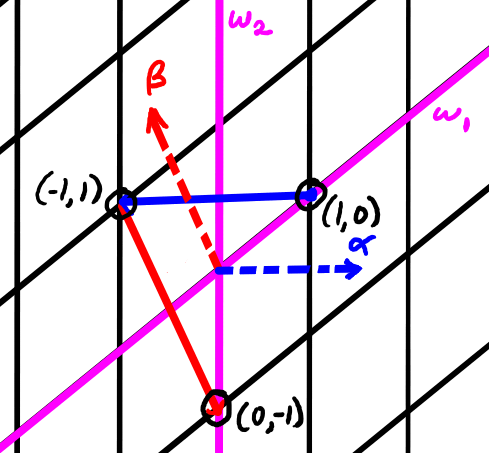
\includegraphics{2018/11/20181122_s1-0.png}
    \caption{The weight lattice for $R_{(1,0)}$. The fundamental weights $\omega_{(1)},\omega_{(2)}$ are the axes in magenta, such that the coordinates $(\lambda_1,\lambda_2)$ correspond to weights $\lambda=\lambda_1\omega_{(1)}+\lambda_2 \omega_{(2)}.$ The roots $\alpha,\beta$ are depicted in blue and red respectively. Arrows connect the highest weight element $\Lambda=\omega_{(1)}=(1,0)$ to the other two weights of this representation.}
    \label{fig:s1-0}
\end{figure}

\begin{figure}
    \centering
    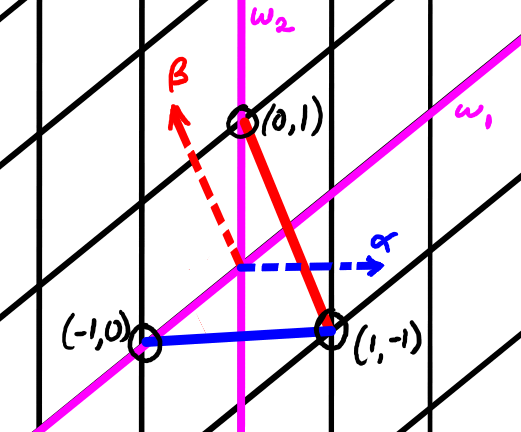
\includegraphics{2018/11/20181122_s0-1.png}
    \caption{The weight lattice for $R_{(0,1)}$. Arrows connect the highest weight element $\Lambda=\omega_{(2)}=(0,1)$ to the other two weights of this representation.}
    \label{fig:s0-1}
\end{figure}

\begin{figure}
    \centering
    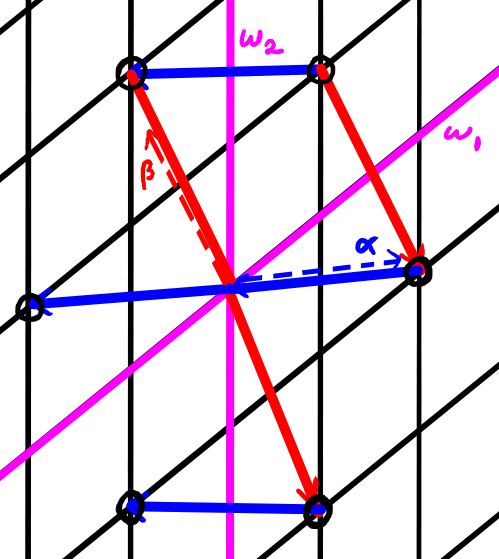
\includegraphics{2018/11/20181122_s1-1.png}
    \caption{The weight lattice for $R_{(1,1)}$. Arrows connect the highest weight element $\Lambda=\omega_{(1)}+\omega_{(2)}=(1,1)$ to the other weights of this representation. As it turns out, our algorithm cannot tell us that there are actually two elements of weight zero, which we need to complete the octet of weights. More sophisticated counting arguments can tell us what the correct multiplicity of each weight is, but we will not be too concerned with them for now}
    \label{fig:s1-1}
\end{figure}

\subsection*{Irreps of $A_2$} For each \term{dominant integral weight}
$$\Lambda=\Lambda^1 \omega_{(1)}+\Lambda^2 \omega_{(2)} \in \bar \cL_W$$
with $\Lambda^1,\Lambda^2 \in \ZZ_{\geq 0}$, we get an irrep denoted $R_{(\Lambda^1,\Lambda^2)}$. As it turns out (cf. Osborn pg. 113), the dimension is given by
$$\dim R_{(\Lambda^1,\Lambda^2)}=\frac{1}{2}(\Lambda^1+1)(\Lambda^2+1)(\Lambda^1+\Lambda^2+2).$$

Note that if $\Lambda_1\neq \Lambda_2$, then we get a conjugate pair of repns of $L(SU(3))$ of the same dimension,
$$R_{(\Lambda^2,\Lambda^1)}=\bar R_{(\Lambda^1,\Lambda^2)},$$
where we send each of the $\lambda \in S_{(\Lambda^1,\Lambda^2)}\mapsto -\lambda \in S_{(\Lambda^2,\Lambda^1)}.$

Our formula tells us the results in Table \ref{tab:a2irreps}.
\begin{table}[]
    \centering
    \begin{tabular}{c|c}
        \\\hline
         $R_{(0,0)}$ & \underline{1} (trivial) \\ \hline
         $R_{(1,0)}$ & \underline{3} (fundamental) \\ \hline
         $R_{(0,1)}$ & $\overline{\underline{3}}$ (anti-fundamental) \\ \hline
         $R_{(2,0)}$ & $\underline{6}$ \\ \hline
         $R_{(0,2)}$ & $\overline{\underline{1}}$ \\ \hline
         $R_{(1,1)}$ & \underline{8} (adjoint) \\ \hline
         $R_{(3,0)}$ & \underline{10} \\ \hline
         $R_{(0,3)}$ & $\overline{\underline{1}}$
    \end{tabular}
    \caption{The irreps (irreducible representations) of the Lie algebra $A_2$.}
    \label{tab:a2irreps}
\end{table}
Now for instance we could take $R_{(1,1)}$ with highest weight $\Lambda=(1,1)$. Thus $(\omega_{(1)}+\omega_{(2)}\in S_{(1,1)}$. Then
$\Lambda-\alpha_{(1)},\Lambda-\alpha_{(2)}\in S_{(1,1)}.$
Thus
$$(1,1)-(2,-1)=(-1,2)\in S_R$$ and $$(1,1)-(-1,2)=(2,-1)\in S_R.$$ Applying the algorithm again, there are also points at
$$\Lambda-\a_{(1)}-\a_{(2)},\Lambda-\a_{(1)}-2\a_{(2)},\Lambda-2\a_{(1)}-\a_{(2)}\in S_R.$$
If we draw this, we get a very nice diagram whose vertices are characterized by the points on a hexagon-- see Fig. \ref{fig:s1-1}. As it turns out, what our algorithm cannot tell us is that there are two elements of zero weight.

Note that finding these weights is a critical task when we are looking at the representation theory of physical systems, since the weights correspond to the quantum numbers of particles! This hexagon looks suspiciously like the Eightfold Way proposed by Murray Gell-Mann.

\subsection*{Tensor products} Let $R_\Lambda,\tilde R_{\Lambda'}$ be irreps of $\fg$ with representation spaces $V_\Lambda$ and $\tilde V_{\Lambda'}$ respectively. As usual, they have weight space decompositions, so we can write them as direct sums:
$$V_\Lambda =\bigoplus_{\lambda\in S_\Lambda}V_\lambda$$
where $R_\Lambda$ has a weight set $S_\Lambda$, and similar for $\tilde R$,
$$\tilde V_{\Lambda'} =\bigoplus_{\lambda;\in \tilde S_{\Lambda'}}\tilde V_{\lambda'}.$$
Now if $\lambda \in S_\Lambda$ and $\lambda'\in \tilde S_{\Lambda'}$ then $\lambda+\lambda'\in L_W[\fg]$ is a weight of the tensor product representation
$$R_\Lambda \otimes \tilde R_{\Lambda'}.$$
\begin{proof}
For an eigenvector $v_\lambda \in V_\lambda$ an eigenspace of $V$, $v_\lambda$ is an eigenvector of the repn $R_\Lambda$ of the Cartan subalgebra generators $H^i$:
$$R_\Lambda(H^i)v_\lambda=\lambda^i v_\lambda.$$
Similarly,
$$\tilde v_{\lambda'}\in \tilde V_{\lambda'}\implies \tilde R(H^i)\tilde v_{\lambda'} = \lambda'{}^i \tilde v_{\lambda'}.$$
Now we recall that the tensor product representation is defined as the representations acting on the vectors in each space:
\begin{align*}
    (R_\Lambda \otimes \tilde R_{\Lambda'}(H^i)(v_\lambda\otimes \tilde v_{\lambda'}&= R_\Lambda (H^i)v_\lambda \otimes \tilde v_{\lambda'}
    +v_\lambda \otimes \tilde R_{\Lambda'}(H^i)\tilde v_{\lambda'}\\
    &=(\lambda+\lambda')^i(v_\lambda\otimes \tilde v_{\lambda'}).
\end{align*}
Hence the weight set $R_\Lambda \otimes \tilde R_{\Lambda'}$ is all such combinations of weights,
$$S_{\Lambda\otimes \Lambda'}=\set{\lambda+\lambda':\lambda\in S_\Lambda, \Lambda' \in \tilde S_{\Lambda'}}.$$
\end{proof}
For finite-dimensional simple complex $\fg$, we can write the tensor product as a direct sum
$$R_\Lambda \otimes R_{\Lambda'} =\bigoplus \mathcal{N}_{\Lambda,\Lambda'}^{\Lambda''}R_{\Lambda''}.$$
These coefficients $\mathcal{N}$ are the multiplicities of these other representations, if you like. As such, $\mathcal{N}_{\Lambda,\Lambda'}^{\Lambda''}\in \ZZ_{\geq 0}$. In fact, they are either $1$ or $0$.

\begin{exm}
Let's sketch an example-- for $\fg=A_2$, we consider the tensor product
$$R_{(1,0)}\otimes R_{(1,0)}.$$
The weight set is
$$S_{(1,0)}=\set{\omega_1,\omega_2-\omega_1,-\omega_2}.$$
The tensor product is the sum of the two weight sets,
$$S_{(1,0)\otimes (1,0)}=S_{(1,0)}+S_{(1,0)}.$$
This is the same game we played when we considered tensor products of angular momentum, except now we are in $L(SU(3))$ so the possibilities live in a higher-dimensional space. What we find is that the new weight set is (just by taking sums of pairs of elements)
$$S_{(1,0)\otimes (1,0)}=\set{2\omega_1,\omega_2,\omega_1-\omega_2,\omega_2,2(\omega_2-\omega_1),-\omega_1,\omega_1-\omega_2,-\omega_1,-2\omega_2}.$$
\end{exm}

\subsection*{Non-lectured aside: weights, roots, and lattices} I know I don't normally do non-lectured asides for this course since the notes and lecturing are extremely thorough, but let me take a minute to discuss some of the terminology we've been playing with here and put them into context.

Before we ever began Cartan classification, we talked about weights. We introduced weights in the context of $L(SU(2))$, where there was one special element $H$ such that $R(H)$ was diagonalizable, and said that the weights were simply the eigenvalues of the matrix $R(H)$. That is, if $R(H)$ has eigenvectors $v_\lambda$, then for
$$R(H)v_\lambda =\lambda v_\lambda,$$
we call these eigenvalues $\lambda$ the weights of the representation.

In hindsight, we recognize that $H$ was just the one-element Cartan subalgebra for $L(SU(2)).$ We defined the Cartan subalgebra $\fh$ as a very special subalgebra of the full Lie algebra $\fg$, which was the maximal abelian subalgebra of $\fg$ where all elements in $\fh$ are ad-diagonalizable (i.e. for every element $H$, the eigenvectors of the ad map $\ad_H$ form a complete basis for the Lie algebra $\fg$).

This leads us to generalize the concept of weights when the Cartan subalgebra has more than one element. In general, the weight set of a representation $R$ is all eigenvalues $\lambda_i$ such that
$$R(H^i)v_{\lambda_i}=\lambda_i v_{\lambda_i}$$ for some element $H^i\in \fh$. Thus it only makes sense to discuss the weights in the context of a specific representation.

Moreover, the elements of the Cartan subalgebra had basis elements $H^i, i=1,\ldots,r$, such that a general element $H\in \fh$ can be written as $H=e_i H^i$ for $e_i\in \CC$. The ad map corresponding to these basis elements, $\ad_{H^i}: \fg\to \fg$, had sets of eigenvalues $\alpha^i$ corresponding to a set of eigenvectors $E^\alpha \in \fg$, such that
$$\ad_{H^i}(E^\alpha)=\alpha^i E^\alpha.$$ 

Here, $\alpha$ is doing double duty as both a \emph{label on the eigenvectors $E^\alpha$} and as a \emph{length-$r$ complex vector representing the eigenvalues of the ad map $\ad_{H^i}$ with $i=1,\ldots,r$}. We called these objects \term{roots}. Using the language we introduced later, we can also say that the roots are the weights of the adjoint representation. 

We then interpreted these roots as elements of the dual space to the Cartan subalgebra, $\fh^*$. That is, an element $\alpha$ is a linear map on the general elements $H=e_i H^i$ in the Cartan subalgebra $\fh$, such that if $H=e_i H^i$, then $$\alpha(H)=\alpha_i e^i \in \CC$$ We can make a similar construction for the weights of a general representation-- for instance, if $R$ is some representation then the elements of the Cartan subalgebra correspond to some maps $R(H^i)$ so that if
$$R(H^i)v_{\lambda_i}=\lambda_i v_{\lambda_i},$$
and $H$ is as before, $H=e_i H^i$, then $$\lambda(H)=\lambda_i e^i.$$
So indeed the weights $\lambda$ are also elements of the dual space $\fh^*$.

We then refined these ideas by arguing that the roots had a well-defined inner product given by the Killing form $\kappa^{-1}$ and therefore a geometry, and moreover we could separate the roots into a set of positive and negative roots $\Phi_+,\Phi_-$. We defined the simple roots as a set of roots $\Phi_S$ such that $\alpha,\beta\in \Phi_S\implies \alpha-\beta \notin \Phi$. We did this in order to find a nice set of linearly independent basis vectors for the dual space, and argued that taking integer linear combinations of the simple roots traces out a root lattice in $\fh^*$.

From the simple roots, we got the simple coroots, which are just the simple roots after a normalization:
$$\alpha^\vee_{(i)}=\frac{2\alpha_{(i)}}{(\alpha_{(i)},\alpha_{(i)})}.$$ Then we can consider the dual of these simple coroots under the inner product. These are a set of elements $\omega_{(i)}$ such that
$$(\omega_{(j)},\alpha^\vee_{(i)})=\delta_{ij}.$$ We call these elements the fundamental weights. The fundamental weights now trace out their own lattice after taking integer linear combinations, known quite sensibly as the weight lattice. Thus the weight lattice is dual to the coroot lattice, and essentially by definition, the Cartan matrix $A^{ij}$ tells us precisely the relationship between the simple roots and the fundamental weights:
$$\alpha_{(i)}=\sum_{j=1}^r A^{ij}\omega_{(j)}.$$

Finally, given a particular irrep $R_\Lambda$, there must be a highest weight
$$\Lambda=\sum_{i=1}^r \Lambda^i \omega_{(i)}$$
where these $\Lambda^i$ are called Dynkin labels. In words, these are simply the coordinates of $\Lambda$ interpreted as a vector in the basis of the fundamental weights $\omega_{(i)}$. Since $R_\Lambda$ is an irrep, we can reach all the other weights of the irrep by subtracting off positive integer multiples of the simple roots.